\documentclass[../main.tex]{subfiles}
\begin{document}

\chapter{Principles of Machine Learning}
\label{sec:second}
\todo[inline]{Hot topic ml}
There is a lot of publicity and promotion regarding machine learning, nevertheless the recognition is well deserved. People working within multiple fields of sciences like computer science, mathematics, statistics and others, most likely know a bit or a lot of machine learning, but how does machine machine learning actually work and what are the wonders of it? 

The main principles of machine learning are quiet straight forward and intuitive. There are multiple forms of machine learning, supervised learning is one of them. The goal of supervised learning is to create models that aim to learn trends from data that can be generalized to predict other unseen data. In search of the perfect generalisation of data, machine learning models need to adjust to training data by optimizing the model, decreasing some loss computed from prediction estimates and true labels. Another form of machine learning is reinforcement learning looking to improve a model based on prior calculations and observations by rewarding and punishing the model based on correct and wrong estimates. For instance one could use reinforcement learning to train an AI agent to master a game like chess or checkers by simulating multiple games, generating skills each game simulated. There is also unsupervised learning which can be recognized as supervised learning without labeled data. Since the data is not labeled, the goal of unsupervised learning is primarily to decide unknown patterns in data. Even though the three presented directions within machine learning are based on different methods, there are multiple common features, for instance they all need to optimize the models in addition to define some loss function to assess the prediction.

In general, the key elements of creating a machine learning model is the dataset if data is needed, labeled or unlabeled. An optimization algorithm used to optimize the machine learning parameters. And of course a chosen machine learning algorithm. In this chapter the key elements of machine learning will be presented along with some machine learning algorithms.

\section{Supervised learning algorithms}
\label{sec:supervised_learning}
\subsection{Linear regression}
The most common supervised learning method is called linear regression, where the name hints about its purpose: finding linear relationships between input data and target values. A more mathematical representation of linear regression is to express the true value \ensuremath{\mathbf{y}} as follows:

\begin{equation}
    \mathbf y=\mathbf X\mathbf \beta+\mathbf \epsilon
    \label{eq:linear regression}
\end{equation}

Where $\epsilon$ is the statistical noise in the dataset, which can be described by random irregularities in the data. Noise in machine learning models are crucial to ensure that the model does not overfit. Which takes us to another important definition in machine learning- overfitting. Overfitting is when a model is fitted so well to training data that it does not longer generalize well on new unseen data, this prevents the model from predicting as good as possible on new unseen data. \ensuremath{\mathbf{X}} is the design matrix of shape $p$ $\times$ $n$ with $p$ being the number of features and $n$ the number of samples. $\mathbf\beta$ is the coefficients which is optimized when training a model. The true value of a single sample can then be expressed by the following expression:

\begin{equation*}
    y=\beta_0+x_1\beta_1+x_2\beta_2...+x_{p}\beta_p+\epsilon
\end{equation*}

In search of the best generalization making the finished model able to be applied on new unseen data predicting the value, one needs to train the model. Training the model is done by optimizing the coefficients \ensuremath{\boldsymbol{\beta}=[\beta_0, \beta_1,..,\beta_p]^T} where $\beta_0$ is the intercept often referred to as the bias. The coefficients is computed as follows by minimizing some loss function $L(\beta)$:

\begin{equation}
  \hat{\mathbf \beta} = \underset{\beta}{\arg \min}\ L(\beta),
\end{equation}

Which defines the final prediction of a single sample as:

\begin{equation}
    \hat{y}=\hat{\beta}_0+x_1\hat{\beta}_1+x_2\hat{\beta}_2...+x_{p}\hat{\beta}_p
    \label{eq:linear regression 2}
\end{equation}

Some loss functions will be presented in \autoref{sec:optimization}.

\subsubsection{The design matrix}
When utilizing different regression methods not only when performing linear regression, but within lots of supervised learning methods, it is important to sort the data into a well designed system for easy access and easier calculations. This is done by sorting the data into a so called design matrix $\textbf{X}$. A design matrix can be left looking the following way, where each row represent one sample:

\begin{equation*}
\mathbf X=  \begin{pmatrix}
   1& x_0^{(0)} & x_1^{(0)} & \ldots & x_{p}^{(0)}\\
   1& x_0^{(1)} & x_1^{(1)} & \ldots & x_{p}^{(1)}\\
     &  &  & \vdots & \\
    1& x_0^{(n)} & x_1^{(n)} & \ldots & x_{p}^{(n)}\\
 \end{pmatrix}
\end{equation*}

By having different coefficients often referred to as weights $\beta$ in front of each term of the design matrix as in \autoref{eq:linear regression 2}, it is possible to calculate how much each element of the design matrix should affect the computations in order to make the best approximations. Following \autoref{eq:linear regression} the predictions can be expressed as a matrix the following way:

\begin{frame}
\footnotesize
\setlength{\arraycolsep}{2.5pt} % default: 5pt
\medmuskip = 1mu % default: 4mu plus 2mu minus 4mu
\begin{equation*}
  \hat{\mathbf y}=  \begin{pmatrix}
    \epsilon_0 & \beta_0 & \beta_1 x_1^{(0)} &  \beta_2 x_2^{(0)} & \ldots &  \beta_p x_{p}^{(0)}\\
    \epsilon_1 & \beta_0 & \beta_1 x_1^{(1)} &  \beta_2 x_2^{(2)} & \ldots &  \beta_p x_{p}^{(1)}\\
     &  &  &  & \vdots & \\
    \epsilon_{n} & \beta_0 & \beta_1 x_1^{(n)} &  \beta_2 x_2^{(n)} & \ldots &  \beta_{p} x_{p}^{(n)}\\
 \end{pmatrix}.
\end{equation*}
\end{frame}

\subsection{Logistic regression}
\label{sec:logreg}
Logistic regression is a method for classifying a set of input variables \ensuremath{\boldsymbol{x}} to an output or class \ensuremath{y_i, i=1,2, \ldots,K} where $K$ is the number of classes. The review in this section is based on Hastie et al. \cite[ch.~4]{HastieTrevor2009EoSL}, and the reader is referred to this book for a more detailed explanation of the topic.

When classifying data, one distinguishes between hard and soft classifications, the former places the input variable into a class deterministically while the latter is a probability that a given variable belongs to a certain class. The logistic regression model is given on the form

\begin{align*}
    \begin{split}
        \log\frac{p(G=1|X=x)}{p(C=K|X=x)}&=\beta_{10}+\beta_1^Tx \\
        \log\frac{p(G=2|X=x)}{p(C=K|X=x)}&=\beta_{20}+\beta_2^Tx \\
        &\vdots\\ 
        \log\frac{p(G=K-1|X=x)}{p(C=K|X=x)}&=\beta_{(K-1)0}+\beta_{K-1}^Tx
    \end{split}
\end{align*}

With $K$ possible classes.

Considering a binary, two-class case with \ensuremath{y_i \in [0,1]}. The probability that a given input variable $x_i$ belongs to class $y_i$ is given by the Sigmoid-function (also called logistic function):

\begin{align*}
    p(x) = \frac{e^x}{1+e^x}=\frac{1}{1+e^{-x}}
    \label{eq:sigmoid}
\end{align*}

A set of predictors \ensuremath{\boldsymbol{\beta}}, which is to be estimated from data then gives the probabilities:

\begin{align*}
    p(y_i=1|x_i,\boldsymbol{\beta})&=\frac{e^{\boldsymbol{\beta}^Tx_i}}{1+e^{\boldsymbol{\beta}^Tx_i}}=\frac{1}{1+e^{-\boldsymbol{\beta}^Tx_i}} \\
    p(y_i=0|x_i,\boldsymbol{\beta})&=1-p(y_i=1|x_i,\boldsymbol{\beta})
\end{align*}

Firstly defining the set of all possible outputs in a data set \ensuremath{\mathcal{D}(\boldsymbol x,\boldsymbol y)}, and assuming that all samples \ensuremath{\mathcal{D}(x_i,y_i)} are independent and identically distributed. The total likelihood can be approximated for all possible outputs of \ensuremath{\mathcal{D}} by the product of the individual probabilities \cite[p.~120]{HastieTrevor2009EoSL} of a specific output $y_i$:

\begin{align}
    P(\mathcal{D}|\boldsymbol{\beta}) = \prod_{i=1}^n[p(y_i=1|x_i\boldsymbol{\beta})]^{y_i}[1-p(y_i=1|x_i,\boldsymbol{\beta})]^{1-y_i}
    \label{eq:likelihood}
\end{align}

\subsection{Nearest Neighbours}
\label{sec:knn}
\todo[inline]{This Nearest Neighbours section is just taken from the special curriculum. Remove or keep section?}
Nearest neighbours, most known as k-nearest neighbours is a powerful and intuitive method which are still widely used even though its simplicity. As the name describes, k-nearest neighbours is based on classifying datapoints based on their nearest neighbours. The $k$ in the name is the amount of neighbours that are going to help predict the category of a datapoint. 

The method is best understood intuitively when imagining a two dimensional graph with datapoints spread around. Each datapoint belongs to one of two categories also called classes, where the category of each datapoint is known. The method is just as useful having more than two categories, but for simplicity only two categories are considered. By inserting an unknown datapoint which is to be classified within one of the two categories, k-nearest neighbours method is applied. For example by having $k=5$, the five nearest neighbours will decide the category of the unknown datapoint. The category that most of the five nearest neighbours belongs to, will be the resulting category of the unknown datapoint.

The method can also be used by having all samples contribute to their category. This way the samples receives weights depending on how close the samples are to the new unknown sample by computing the squared distance. The method is often called nearest neighbours when all samples affect the outcome of a single sample used, since then $k$ equals the entire dataset. The weights are given by:
\begin{equation}
    \omega_i=1-\frac{1}{c}|\hat{x}-x_i|^2
\label{eq:knnweight}
\end{equation}
Where \ensuremath{\hat{x}} is the unknown sample, \ensuremath{x_i} is the $i$'th sample and $c$ is a constant. By computing the weights of all the samples, the probability of classifying the unknown datapoint within category \ensuremath{y}, which is an arbitrary category label from the dataset, can be computed by the following:
\begin{equation}
    p_{\hat{x}}(\hat{y}=y)=\frac{1}{\chi}\frac{1}{M_y}\sum_{i|y_i=y}\omega_i
    \label{eq:knnprob}
\end{equation}
Where \ensuremath{M_y} is all the training inputs labeled withing category \ensuremath{y} and \ensuremath{\frac{1}{\chi}} is a normalisation constant. The category with the highest probability naturally labels the unknown sample.

\subsubsection{Application of nearest neighbours}
\label{KNNimp}
A demonstration of the nearest neighbours method utilized in a classical case will be shown, in addition to a quantum nearest neighbours method later i the thesis, both applied to the same dataset.

The example is based on the example found in \cite[ch.~1]{10.5555/3309066}. The dataset that is going to be used are some few samples from the titanic dataset. The dataset can be found at the well known dataset publisher kaggle \cite{cite:kaggletitanic}. The dataset is known as the titanic dataset, which is based on the survival of the passengers on the titanic. Info like age, cabin number, sex, number of siblings and such is published. The goal of the following example is to place the passengers within two categories, survivor or not a survivor.

To focus on the beauty of the algorithm only three samples will be used. Three samples are quiet obviously too few to be reliable in real implementations. Only two properties from the dataset will be used, the price of the cabin and the ticket number. The survival of two of the samples are already known, while the last sample are going to be classified as survied or not survived. The small sample dataset from \cite[ch.~1]{10.5555/3309066} can be seen in table \ref{tab:dataset_tit}.

\begin{table}[ht]
\caption{Table showing some samples used for creating a small dataset. The dataset is showing the ticket price the travelers paid and the room number before normalisation(BN), and the same information after normalisation(AN) assuming the maximum ticket price and room number was 10000 and 2500 respectively. The survival column shows the survival of the travelers, 1 means survival while 0 means no survival.}
\centerline{
\begin{tabular}{ cccccc } 
\toprule
Traveler & Price (BN)& Room number (BN) & Price (AN) & Room number (AN) & Survival \\
\midrule
1        &   8500 & 0910 & 0.85 & 0.36 & 1\\
2        &   1200 & 2105 & 0.12 & 0.84 & 0\\
3        &   7800 & 1121 & 0.78 & 0.45 & \\
\bottomrule
\end{tabular}}
\label{tab:dataset_tit}
\end{table}

By plotting the data of the travelers the classification is quiet easy with so a few samples. The plot can be seen in figure \ref{fig:classicknn}, which easily shows that the unknown traveler will be classified as a survivor.

\begin{figure}[ht]
    \centering
    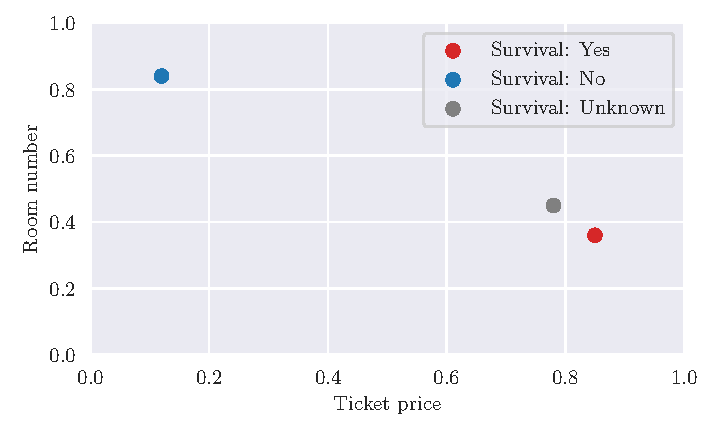
\includegraphics{figures/Cknn.pdf}
    \caption{Plot of the ticket price and room number for the three travelers.}
    \label{fig:classicknn}
\end{figure}

Even though we know the classification, we still want to compute the probability of classifying the unknown sample within the two categories to have a closer look at the comparison with the quantum nearest neighbours later in the thesis. The probability is computed by using equation \ref{eq:knnweight} and \ref{eq:knnprob}. The outcome of the computations results in a probability of classifying the unknown sample as a survivor to be 0.522, while the probability of classifying the same sample as a traveler that did not survive is 0.478.

\subsection{Dense neural networks}
Neural networks is a machine learning method which is roughly made up of the perception of how the real brain works. Neural networks are created by having an input layer, output layer and one or more hidden layers between. Each layer consists of one or more nodes, often referred to as neurons. In a dense neural network, each of the nodes are connected to each node in the layer in front and behind. A visual explanation of a neural network can be seen in \autoref{fig:nnimg}.\\

\begin{figure}[h]
    \centering
    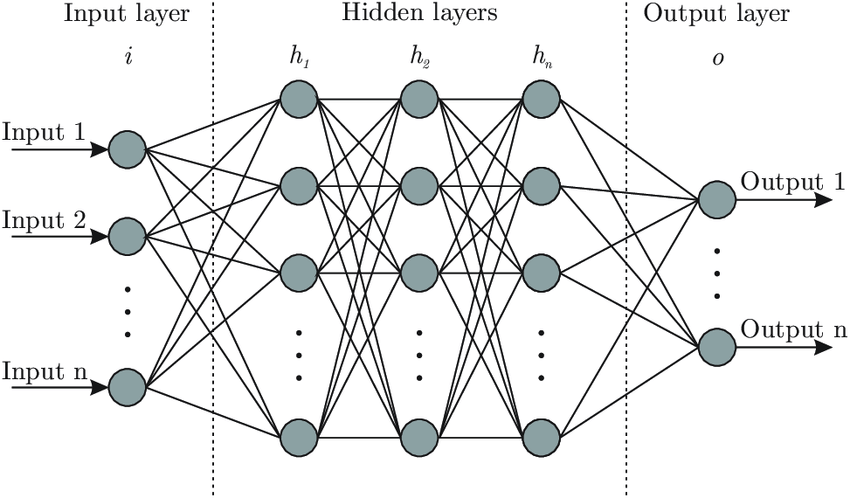
\includegraphics[width=0.8\textwidth]{figures/neuralnet.png}
    \caption{Schematic diagram of a dense neural network consisting of up to n hidden layers and nodes. Note that all layers are fully connected.
 Figure from \cite{cite:nnfig}}
    \label{fig:nnimg}
\end{figure}

Roughly explained each node in the neural network has a corresponding weight which is tunable just like the coefficients $\beta$ in the earlier sections. The goal of a neural network is to adjust these weights during training of the network to make a certain prediction based on the input data. 

Feed forward neural networks which was one of the first and most simplistic types of artificial neural networks \cite{Schmidhuber_2015} is defined by having the information in the neural network only go in one direction without creating cycles of information-flow within the network, therefore the information either goes forward during prediction or backward during weight updates.

The feed forward part of the network is done by inserting input values in the first layer. The values of the neurons in the layer in front, also called activation's are computed, then the neurons in each layer are computed all the way to the activaton(s) in the output layer which serves as the final prediction of the network. It is most common to wrap a non linear activation function around each node in addition to adding a potential bias to the node. By using a non linear activation function around the nodes, the network layers have the possibility to go from linear layers to non linear layers. The activation of layer $l$ are left looking as follows:

\begin{equation}
    \boldsymbol{a}^l=f^l(W^l\boldsymbol{a}^{l-1}+\boldsymbol{b}^l)
\label{eq:activation}
\end{equation}

Where \ensuremath{W} is the weight matrix, $b$ is the bias and \ensuremath{f(x)} is the activation function used, making the neural network non-linear. There are several popular activation functions, with sigmoid-, ReLU- and tanh function being some of the most common ones \cite{activation_cunctions_citation}. The activation function is often selected based on the issue the neural network are going to overcome, in addition it is important to keep the derivative of the activation functions in mind, due to the possibility of having exploding and vanishing gradients. An overview of some popular activation functions can be seen in \autoref{tab:activaton_functions2}

\begin{table}[h!]
\centering
\caption{A variety of activation functions, commonly used in neural networks}
\begin{tabular}{c c} 
\hline
Name  & Activation Function \\
\hline
Identity  & $f(x)=x$ \\
Sigmoid  & $f(x)=\frac{1}{(1+e^{-x})}$ \\
Tanh  & $f(x)=\frac{e^x-e^{-x}}{e^x+e^{-x}} $ \\
Leaky Relu  & $f(x)=\max(0.01x, x)$ \\
\end{tabular}
\label{tab:activaton_functions2}
\end{table}

By adding more layers and making the neural network deeper, the computational complexity naturally also increases. Due to the increase in computational complexity, there is a lot of variations within neural networks to ease the computations without loosing too much of the power of dense neural networks, e.g. convolutional neural networks, recurrent neural networks and many more.

\subsubsection{Backpropagation}
The widely used training method for a lot of variations of neural networks are called backpropagation. Backpropagation is used to update the weights in a neural network, by differentiating backward in a neural network. When training models with machine learning, a loss- or a cost function is defined as a measurement of how good the network is performing.

To calculate new and more optimized weights, the loss function needs to be minimized, which naturally opens up the need for a gradient. The gradient of the loss function with respect to the weights and bias are calculated by using the aforementioned backpropagation utilizing the chain rule. This method revolves around calculating the gradient one layer at a time, starting with the last layer's activation(s) and moving backwards layer by layer, therefore the name of the algorithm. The gradients are continued to be computed through the neural network structure to find the final gradient.

The training regime goes as follows, starting of with some data fed forward into the dense neural network which then predicts the output \ensuremath{a^{last}} in the last layer. Which then is used to calculate the loss \ensuremath{L(a^{last},y)}, where y is the target value. The prediction will certainly have some error defined by the loss function. Which then are optimized by using some optimization technique, which will be presented in section \cref{sec:optimization}.

The gradient is computed by using the chain rule and \autoref{eq:activation} to express the activation's in the prior layers \cite[ch.~7]{rojasRa:nnsystematic} \cite{chain_rule}, and recursively computing the gradients backward into the net. The derivative of some node with respect to some weight and some bias can be written as follows respectively, the derivation can be seen in the appendix:

\begin{align*}
\frac{L\left(\boldsymbol{a}^{last}, \boldsymbol{y}\right)}{\partial W_{i j}^{l}}&=z_{i}^{l} \frac{\partial a_{i}^{l}}{\partial W_{i j}^{l}} \\
\frac{L\left(\boldsymbol{a}^{last}, \boldsymbol{y}\right)}{\partial b_{i}^{l}}&=z_{i}^{l} \frac{\partial a_{i}^{l}}{\partial b_{i}^{l}}
\end{align*}

Where \ensuremath{z_i^l} is given as the following:

\begin{equation*}
    z_i^l= \frac{\partial L(a^{last},y)}{\partial a_{i}^l}= \sum_n z_n^{l+1}\frac{\partial a_n^{l+1}}{\partial a_{i}^l}
\end{equation*}

Which shows how the gradients of activation of nodes in the same layers are summed up and being used in the calculations of the gradients of the layers closer to the input layer in dense neural networks.

\section{The Boltzmann machine}
\label{sec:BM}
The Boltzmann machine was proposed by Geoffrey Hinton and Terry Sejnowski in 1985 and led on to a massive interest in Boltzmann machines at the time being\cite{ACKLEY1985147}. Boltzmann machines are unsupervised machine learning networks using an undirected graph structure to process information \cite{VQB:litteraturelist}. The network is often referred to as a stochastic recurrent neural network, which is able to learn probability distributions over a set of inputs\cite{Hinton:2007}. The reason that Boltzmann machines are stochastic, is because the decision on a node being on or off is made stochastic. Boltzmann machines consists of visible and hidden nodes, and often biases. The Boltzmann machine is often easier to grasp for the reader after having a look at the schematic structure first, which can be seen in \autoref{fig:BM structure}. All nodes is connected to each other, where the connections are the essence of the network. The connections between the nodes are also called weights, and are used to store prior learned knowledge\cite{VQB:litteraturelist}. The connections have varying strengths which means that the training of Boltzmann machines are based on optimizing these same weights, until the given input results in the desired output with high probability.

\begin{figure}[h]
    \centering
    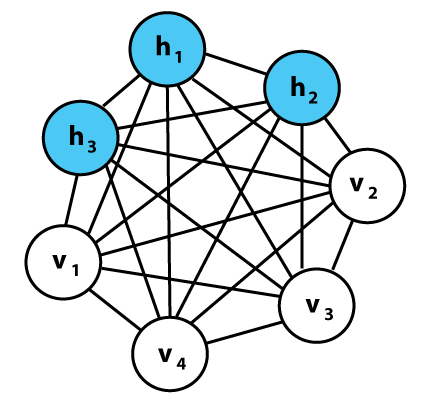
\includegraphics[width=0.5\textwidth]{figures/Boltzmannexamplev1.png}
    \caption{Architecture of a Boltzmann machine, having every node connected to each other. This Boltzmann machine consists of four visible nodes and three hidden nodes. Figure from \cite{BMfig}}
    \label{fig:BM structure}
\end{figure}

Having a look at the stochastic dynamics of Boltzmann machines presented in \cite{Hinton:2007}, some mathematical formulas need to be presented. First of all a unit $z_i$ can be turned on or off, representing binary states usually $z_i\in\{-1,1\}$ or $z_i\in\{0,1\}$. The visible and hidden nodes at a certain configuration $\mathbf{z}=\{\mathbf{v},\mathbf{h}\}$ is then used to compute the energy of the system in a certain configuration by using the following formula, summing through each hidden- and visible node:

\begin{equation*}
    E(\mathbf{z}; \theta) = -\sum_i^N \Tilde{\theta_i}z_i-\sum_{i,j}^N W_{ij}z_iz_j
\end{equation*}

Where $N$ is the number of nodes in the Boltzmann machine, $\theta=\{\Tilde{\theta}, W\}\in\R$ represents the trainable parameters. $W$ is the interaction matrix defining the strength between nodes and $\Tilde{\theta}$ is the bias appended to the nodes.

Updating the nodes consistently until the computations converge, will sooner or later end up with a so called Boltzmann distribution, often called equilibrium distribution. After this the probability of observing a certain configuration of the visible nodes $v$ sampled from the Boltzmann distribution is given by the following formula:

\begin{equation*}
    p(\mathbf{z}; \theta)=\frac{e^{-E(\mathbf{z}; \theta) /\left(\mathrm{k}_{\mathrm{B}} \mathrm{T}\right)}}{Z}
\end{equation*}

With $k_b$ being the Boltzmann constant, T is the temperature of the system. $k_b T$ is quiet often set to be equal to $1$ which will be done in this thesis also, therefore the factor will be left out in future energy equations in the thesis. $Z$ is the so called canonical partition function given as follows:

\begin{equation*}
Z(\mathbf{z}; \theta)=\sum_{v, h}^N e^{-E(\mathbf{z}; \theta)}
\end{equation*}

\subsection{The restricted Boltzmann machine}
A quiet well known feature about Boltzmann machines is that the learning algorithm has the potential to be quiet slow due to a hard time converging towards a final state\cite{Hinton:2007}. A way to deal with this problem is to implement a so called restricted Boltzmann machine instead.

The difference between a regular Boltzmann machine and a restricted Boltzmann machine is that no nodes in the same layer is connected to one another in the restricted one, while in a regular Boltzmann machine nodes usually are connected to all other nodes\cite{BM_book}. The structure of a restricted Boltzmann machine can be seen in \autoref{fig:RBM_structure}.

\begin{figure}[h]
    \centering
    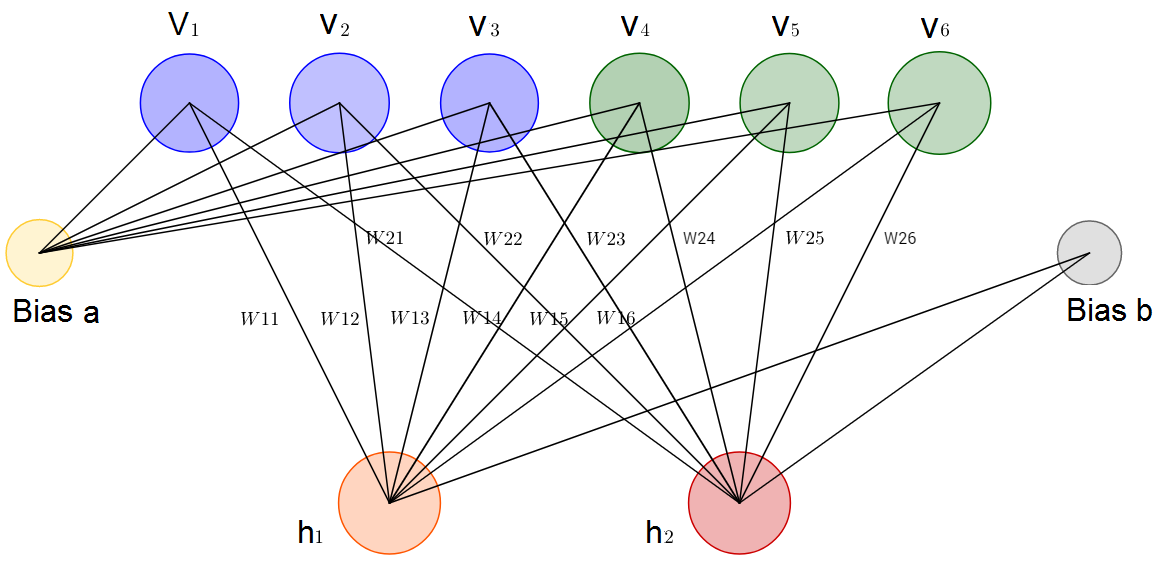
\includegraphics[width=0.8\textwidth]{figures/boltzmann_machine_restricted.png}
    \caption{Architecture of a restricted Boltzmann machine, having the visible nodes connected to every hidden node and the visible bias, while the hidden nodes are connected to all the visible nodes and the hidden bias. The W's in the image is values of the weight matrix which decides how strong the connection between each visible and hidden node is. Figure from \cite{fig_RBM}.}
    \label{fig:RBM_structure}
\end{figure}
\todo[inline]{Should switch out the figure with a nicer one}

\subsubsection{Binary Restricted Boltzmann machine}
RBMs are originally based on binary stochastic visible and hidden variables, with a given energy function of a joint state of visible and hidden nodes looking as follows:

\begin{equation}
E(\mathbf{v}, \mathbf{h}; \theta) =-\sum_{i,j}^{V,H} W_{i j} v_{i} h_{j}-\sum_{i}^V b_{i} v_{i}-\sum_{j}^H a_{j} h_{j}
\label{eq:energfunkeruu}
\end{equation}

With $V$ and $H$ being the number of visible and hidden nodes respectively, $\theta=\{W, \mathbf{b}, \mathbf{a}\}\in\R$ represents the trainable parameters; $W$ being the interaction matrix, defining the strength between visible and hidden nodes, $b$ and $a$ represents the visible and hidden bias respectively. 

One of the wonders of the structure of RBMs is that due to the hidden nodes and visible nodes being bipartite, the joint probability can be written as a marginal probability $p_{v}$ as a sum over hidden nodes as follows\cite{rbm_article}:

\begin{equation*}
    p(\mathbf{v}) =\frac{1}{Z} \sum_{\mathbf{h}}^H \exp ( E(\mathbf{v}, \mathbf{h}; \theta))
\end{equation*}

Which gives the following by inserting the expression of \autoref{eq:energfunkeruu} and factorizing the terms not including any nodes within the exponential outside the sum:

\begin{equation*}
    p(\mathbf{v})=\frac{1}{Z} \exp \left(\mathbf{b}^{\top} \mathbf{v}\right) \prod_{j}^{H} \sum_{h_{j} \in\{0,1\}} \exp \left(a_{j} h_{j}+\sum_{i=1}^{V} W_{i j} v_{i} h_{j}\right)
\end{equation*}

Since $h_j$ only takes takes $\{0,1\}$ as values, the last summation can be written out completely which then gives the final marginal probability:

\begin{equation}
     p(\mathbf{v})=\frac{1}{Z} \exp \left(\mathbf{b}^{\top} \mathbf{v}\right) \prod_{j}^{H}\left(1+\exp \left(a_{j}+\sum_{i=1}^{V} W_{i j} v_{i}\right)\right)
\label{eq:marg_prob}
\end{equation}

To determine and updating the state of a node, a value is chosen stochastically from a conditional probability. The probability of having a hidden node 'on' taking the binary value of 1 is given by the following equation:

\begin{equation}
p\left(h_{j}=1 \mid \mathbf{v}\right)=\delta\left(\sum_{i}^V W_{i j} v_{i}+a_{j}\right)
\label{eq:CP_BH}
\end{equation}

Where $\delta$ is a sigmoid function. The same conditional probability of having a visible node 'on' is given by:

\begin{equation}
p\left(v_{i}=1 \mid \mathbf{h}\right)=\delta\left(\sum_{j}^H W_{i j} h_{j}+b_{i}\right)
\label{eq:CP_BV}
\end{equation}

Even though binary RBMs are useful to such a large degree, sometimes real-valued inputs are preferred over binary inputs. Luckily binary RBMs are easily extended to accept continuous input values.

\subsubsection{Gaussian-Binary Restricted Boltzmann machine}
From time to time binary inputs of RBMs are not always the instinctive input of physical problems, depending on the data. Fortunately RBMs are extended to accept real valued visible inputs quiet straightforwardly. When using real valued visible vectors and binary hidden nodes taking values of $\{0,1\}$ the model is called a Gaussian-Binary Restricted Boltzmann machine due to the visible units embracing a Gaussian distribution, and the hidden nodes being binary. Sometimes this type of RBM is referred to as a Gaussian-Bernoulli RBM. The energy function is given as the following \cite{rbm_article}:

\begin{equation}
E(\mathbf{v}, \mathbf{h} ; \theta)=\sum_{i}^{V} \frac{\left(v_{i}-b_{i}\right)^{2}}{2 \sigma_{i}^{2}}-\sum_{i}^{V} \sum_{j}^{H} W_{i j} h_{j} \frac{v_{i}}{\sigma_{i}}-\sum_{j}^{H} a_{j} h_{j}
\label{eq:energyfunciongauss}
\end{equation}

With $\theta=\left\{W, \mathbf{a}, \mathbf{b}, \sigma \right\}$ being the trainable parameters. $\mathbf{\sigma}$ is the standard deviation. The standard deviation is often predetermined prior to the training.

The marginal probability is then derived the same way as for \autoref{eq:marg_prob}, which gives the following marginal distribution:

\begin{equation*}
P(\mathbf{v} ; \theta)=\sum_{\mathbf{h}} \frac{\exp (-E(\mathbf{v}, \mathbf{h} ; \theta))}{\int_{\mathbf{v}^{\prime}} \sum_{\mathbf{h}} \exp (-E(\mathbf{v}, \mathbf{h} ; \theta)) d \mathbf{v}^{\prime}}
\end{equation*}

With the denominator being the integral over all possible visible states.

The conditional probability of the visible vector taking a value $x$ given a set hidden vector $\mathbf{h}$ is derived from the energy function in \autoref{eq:energyfunciongauss} which gives the following:

\begin{equation}
p\left(v_{i}=x \mid \mathbf{h}\right)=\frac{1}{\sqrt{2 \pi} \sigma_{i}} \exp \left(-\frac{\left(x-b_{i}-\sigma_{i} \sum_{j}^H h_{j} W_{i j}\right)^{2}}{2 \sigma_{i}^{2}}\right)
\label{eq:CP_CV}
\end{equation}

With the conditional probability of a certain hidden node being 'on' given an observed visible vector $\mathbf{v}$ is given as follows:

\begin{equation}
p\left(h_{j}=1 \mid \mathbf{v}\right)=\delta\left(b_{j}+\sum_{i}^V W_{i j} \frac{v_{i}}{\sigma_{i}}\right)
\label{eq:CP_CH}
\end{equation}

With $\delta$ being the sigmoid function.

\subsection{Gibbs sampling}
Due to the objective of training a Boltzmann machine being to represent an intrinsic distribution of provided data, the reconstruction of data is still needed to be done. This is done by sampling from the probability distribution learned by the Boltzmann machine. There are multiple ways of sampling from a learned distribution (e.g. the Metropolis algorithm and the Metropolis-Hastings algorithm), however Gibbs sampling will be utilized in this thesis.

Gibbs sampling is an algorithm based on Markov chain Monte Carlo methods(MCMC). Due to drawing exact quantities from a distribution made by a probabilistic model not always being a walk in the park, MCMC algorithms are therefore used to estimate such quantities. 

A Markov chain is essentially a stochastic process which is based on modelling a discrete sequence of random variables in a system, where the next state of the system is only dependent of the current state\cite{article_rbm2}. A Monte Carlo method on the other hand is used to estimate statistical quantities from drawing samples from a distribution, assumed that samples easily can be drawn from the distribution of relevance. MCMC combines these two methods to draw samples from strenuous-sampled distributions.

Gibbs sampling is an excellent choice of sampling method when dealing with multivariate probability functions in addition to having good access to the conditional distributions. Gibbs sampling is a subcategory of the Metropolis-Hastings algorithm. The essence of Gibbs sampling is to use the conditional distributions to refresh nodes by the probabilities computed, and thereby construct Markov chains following accordingly. Gibbs samples in Boltzmann machines are produced by picking a random node in the network, and updating the node based on the state of the other nodes and the conditional probabilities. The conditional probabilities for binary- and continuous-binary RBMs are given in Equation \ref{eq:CP_BH}, \ref{eq:CP_BV}, \ref{eq:CP_CV} and \ref{eq:CP_CH}.

\begin{comment}
\section{Sampling methods}
\todo[inline]{Only keep this section if I have the time to use the RBM from fys4411, maybe as a subsection of BMs?}
\todo[inline]{Might want to move the sampling methods to the many body section if I write it in connection with moving particles?}

To sample from distributions made by utilizing machine learning methods like the Boltzmann machine, some sampling methods need to be chosen. The sampling methods that are going to be used in this thesis are the Metropolis algorithm, also called brute force sampling, Metropolis-Hastings algorithm also called importance sampling, and Gibbs sampling. 


\subsection{Metropolis Algorithm}
\label{sec:MA}
The Metropolis algorithm is used when proposing and carrying out a step in a Monte Carlo simulation \cite{hanada2018markov}. When choosing a step that a bit of randomness is introduced, that is because the steps are chosen randomly by the following equation:

\begin{equation}
    r^{new}=r^{old}+\in [-0.5,0.5] \cdot dr
\end{equation}

Where dr is a set step length. The step length is multiplied by a random number in the uniform interval [-0.5,0.5], to allow moves along both the positive and negative axis.

After the new step is proposed the decision of acceptance or rejection remains. Calculating the ratio \ensuremath{\phi} and demanding that the ratio is larger than a random variable from the interval [0,1] accepts the step. The ratio is computed as the following:

\begin{equation}
    \phi=\frac{|\Psi(\mathbf{r}^{new})|^2}{|\Psi(\mathbf{r}^{old})|^2}
    \label{eq:ratio}
\end{equation}

Having the steps accepted by the Metropolis algorithm is securing that the simulation and sampling is mainly focused around the largest part of the probability density function, because the ratio can be written as:

\begin{equation}
   \frac{|\Psi(\mathbf{r}^{new})|^2}{|\Psi(\mathbf{r}^{old})|^2}=   \frac{P(\mathbf{r}^{new})}{P(\mathbf{r}^{old})}
\end{equation}
Where $\Psi$ is the wave function.

\subsection{Metropolis-Hastings Algorithm}
\label{sec:MHA}
The Metropolis-Hastings algorithm, also known as importance sampling is an algorithm that can be used instead of the Metropolis algorithm when sampling from distribution. The wave function is contributing to the movement of the particle by a so called drift force \ensuremath{F}, while the Fokker-Planck equation and the Langevin equation is used to produce the route. For a more indepth explanation on Metropolis-Hastings algorithm feel free to have a look here \cite{robert2016metropolishastings}.

The main difference between a usual Metropolis algorithm and the Metropolis-Hasting algorithm is that the later implements a so called drift force which is helping the sampling happen closer towards the largest part of the probability density function(PDF). The drift force \ensuremath{F} is expressed as the following when dealing with wave functions:

\begin{equation}
   F = \frac{2\nabla \Psi}{\Psi}.
 \end{equation}

Further into the Metropolis-Hastings algorithm there is a need for Green's function. The reason for this is that Green's function works as the transition probability contributing to the ratio \ensuremath{\phi} seen in \autoref{eq:ratio}, this way:

\begin{equation}
	\phi=\frac{G(\boldsymbol{r}^{old},\boldsymbol{r}^{new})|\Psi_T(\boldsymbol{r}^{old})|^2}{G(\boldsymbol{r}^{new},\boldsymbol{r}^{old})|\Psi_T(\boldsymbol{r}^{new})|^2}
\end{equation}

Where Green's function is expressed as followed:

\begin{equation}\label{eq:Greens_Function}
	G(\boldsymbol{r}^{old},\boldsymbol{r}^{new})=\frac{1}{(4\pi D \Delta t)^{3/2}}\sum_{i=1}^N \exp \left(-\frac{(\boldsymbol{r}_i^{old}-\boldsymbol{r}_i^{new}-D\Delta t\boldsymbol{F}_i(\boldsymbol{r}^{new}))^2}{4D\Delta t}\right)
\end{equation}
Where D is the diffusion constant and \ensuremath{\Delta t} is the stepstep.

After the new step is proposed the decision of acceptance or rejection remains. Calculating the ratio and demanding that the ratio \ensuremath{\phi} is larger than a random variable from the interval [0,1] accepts the step.

Also in the Metropolis-Hastings algorithm a step is proposed and checked for acceptance, by computing the ratio \ensuremath{\phi} and comparing to some random variable in the uniform interval of $[0,1]$.

The reason for using the Metropolis-Hastings algorithm instead of the Metropolis algorithm is that more steps would be accepted due to the drift force leading toward the center of the PDF.

\subsection{Gibbs sampling}
Gibbs sampling is a method that can be used as an alternative to the Metropolis- and Metropolis-Hastings algorithm. Gibbs sampling is a great choice when dealing with multivariate probability function. By using the following distribution as the wave function, it is possible to model the positional probability distribution:

\begin{equation}
    \Psi_{Gibbs}=\sqrt{F_{rbm(\boldsymbol{X})}}
\end{equation}

Which means that the following formula gives the positional probability distribution:

\begin{equation}
    |\Psi_{Gibbs}|^2={F_{rbm(\boldsymbol{X})}}
\end{equation}
The wave function in both formulas can be seen later in \autoref{eq:wavef}.

In this article Gibbs sampling is sampling from the joint probability of the visible and hidden nodes. The samples are refreshed by setting the hidden nodes to binary values of 0 or 1 by the following formulas derived in \cite{BM_book}:

\begin{equation}
    P(h_J=1|\boldsymbol{X})=\delta(\delta^{input})
\end{equation}

and

\begin{equation}
    P(h_J=0|\boldsymbol{X})=\delta(-\delta^{input})
\end{equation}

Where \ensuremath{\delta(\cdot)} is a sigmoid function and \ensuremath{\delta^{input}} will be defined later in \autoref{sig:input}.

By using the sampled values of the visible nodes, to construct the probability density the positional distribution is received. Efficiency-wise Gibbs sampling is better compared to the Metropolis and the Metropolis Hastings algorithm due to the fact that the acceptance rate is 100\% because the nodes are updated based on the sampled values rather than accepted and rejected, which ensures that Gibbs sampling is using all its computational power on accepted moves.
\end{comment}

\section{Optimizing the supervised learning algorithms}
\label{sec:optimization}

\begin{comment}
From statistical decision theory, the optimal predictor can be derived given a specific loss function $L$.
\end{comment}

So how is it possible to optimize machine learning models to achieve desired results. As explained in \autoref{sec:supervised_learning}, the essence of machine learning depends on optimizing models by finding parameters that give the best predictions applied to unseen data. The process of optimizing parameters towards a complete machine learning model is usually done by finding the parameters giving the lowest loss computed by some loss function $L$. The loss function evaluates how accurate a prediction is. Then by using an optimization technique it is possible to change the parameters in a way that minimizes the loss fitting the model to the data in other words.

\subsection{Some loss functions}

\subsubsection{Mean absolute error}
There are several possible loss functions which determines how good or bad a prediction is. Mean absolute error(MAE) is one of them. The MAE formula goes as follows:

\begin{equation*}
    L(x_i; \boldsymbol{\beta})=\frac{1}{n}\sum_{i=0}^n|y_i-f(x_i; \boldsymbol{\beta})|
\end{equation*}

Where $n$ is the number of samples, $y_i$ is the true label of the \ensuremath{i}'th sample and $f(x_i; \boldsymbol{\beta})$ is the prediction of the sample. MAE is often used when utilizing linear regression. 

\subsubsection{Mean squared error}
Mean squared error(MSE) is one of the most popular loss functions and is normally used when dealing with linear regression, . The formula for MSE goes as follows:

\begin{equation*}
    L(x_i; \boldsymbol{\beta})=\frac{1}{n}\sum_{i=0}^n(y_i-f(x_i; \boldsymbol{\beta}))^2
\end{equation*}

Using MSE penalizes so called outliers in the data to a larger degree compared to MAE due to the difference between the true- and predicted value being squared.

\begin{comment}
\subsubsection{Maximum likelihood estimator and negative log-likelihood}
To maximize the probability function in \autoref{eq:likelihood} introduced in \autoref{sec:logreg} about logistic regression one can use the maximum likelihood estimator(MLE), by taking the logarithm of \autoref{eq:likelihood}, but one usually minimize the negative log-likelihood(NLL) instead to obtain \ensuremath{\boldsymbol{\beta}}:

\begin{equation*}
\begin{split}
    L_{NLL}(\hat{\beta})&=\-log P(\mathcal{D}|\boldsymbol{\beta}) =\\ &-\sum_{i=1}^n[y_i\log p(y_i=1|x_i\boldsymbol{\beta})+(1-y_i)\log(1-p(y_i=1|x_i,\boldsymbol{\beta}))]
    \label{eq:log-likelihood}
\end{split}
\end{equation*}

It is worth mentioning that the NLL function has no analytically minima, which therefore is found numerically. Some numerical minimization algorithms will be presented in \autoref{sec:optimization}.
\end{comment}

\subsubsection{Cross entropy loss}
The cross entropy loss function is a frequently used loss function within machine learning. Cross entropy is based on computing the total entropy between two probability distributions, and is especially common regarding classification problems. The formula for cross entropy goes as follows:

\begin{equation*}
    L(x_i; \boldsymbol{\beta})=-\sum_{i=0}^{n}y_i log(f(x_i; \boldsymbol{\beta})))
\end{equation*}

Where $n$ is the number of probability events.

Cross entropy is often transformed to a binary cross entropy function when dealing with classification between two classes:

\begin{equation*}
    L(x_i; \boldsymbol{\beta})=-\frac{1}{n}\sum_{i=0}^{n}y_i log(f(x_i; \boldsymbol{\beta}))+(1-y_i)log(1-f(x_i; \boldsymbol{\beta}))
\end{equation*}

Which naturally strips away the first or second part of the formula based on the fact that the true label $y_i$ is either zero or one. In addition, by taking the logarithm of the prediction error, the more confident a prediction is, the larger the loss of the sample will be if the prediction is untrue.

\subsection{Finding coefficients in linear regression}
\subsubsection{Ordinary least squares regression}\label{sec:ols}
Ordinary least squares (OLS) regression is one of the most common regression model. To fit a linear model the most popular method is using least squares method, which is based on using the residual sum of squares(RSS) as a cost funtion \cite[ch.~2]{HastieTrevor2009EoSL}. It is worth mentioning that cost- and loss functions often is used interchangeably in some literature, while in reality cost function is some mean of a loss function applied to multiple samples. The RSS function goes as follow:

\begin{equation}
  \label{eq:rss}
  \text{RSS}(\boldsymbol{\beta}) = \sum_{i=1}^n (y_i -  f(x_i; \boldsymbol{\beta}))^2.
\end{equation}

Given $n$ datapoints, sample $x$ and prediction coefficients $\boldsymbol{\beta}$. Due to \cref{eq:rss} being quadratic, the minimum of the function is guaranteed to exist.

The cost function we use for OLS regression is the residual sum of squares (RSS) function:

Finding the optimal parameters $\boldsymbol{\beta}$ by minimizing the RSS is done the following way using matrix notation:

\begin{equation*}
  \text{RSS}(\boldsymbol\beta) = (\mathbf y  - \mathbf X\boldsymbol\beta)^2=(\mathbf y  - \mathbf X\boldsymbol\beta)^T(\mathbf y - \mathbf X\boldsymbol\beta) 
\end{equation*}

Which further on is differentiated with respect to $\boldsymbol\beta$:

\begin{equation*}
  \frac{\partial \text{RSS}}{\partial \boldsymbol\beta} = -2\mathbf X^T (\mathbf y - \mathbf X\boldsymbol\beta) .
\end{equation*}

Where the derivative naturally is set to 0 and used to find the final coefficients:

\begin{equation*}
  \mathbf X^T(\mathbf y -\mathbf X\boldsymbol\beta) = 0
\end{equation*}

If the matrix $\boldsymbol X^T \boldsymbol X$ is non singular hence invertible, the final coefficients can be written as follows:

\begin{equation}
  \hat{\boldsymbol{\beta}} = (\mathbf X^T\mathbf X)^{-1}\mathbf X^T \mathbf y
  \label{eq:rss_ols}
\end{equation}

OLS models are quiet simple compared to other predictive models, hence OLS models has quiet high bias but low variance at the same time. This makes OLS regression at risk of overfitting. Luckily there are other models which ensures higher variance, less bias and less overfitting.

\subsubsection{Lasso regression}
Lasso regression is a shrinking method, which penalizes the prediction coefficients based on the sizes of them by a factor  $\lambda$.

\begin{equation}
  \label{eq:L1_algo}
  \hat{\boldsymbol{\beta}}^{\text{lasso}} = \underset{\beta}{\arg \min} \begin{Bmatrix}\sum_{i=1}^N\left(y_i - \beta_0 - \sum_{j=1}^p x_{ij}\beta_j\right)^2 + \lambda \sum_{j=1}^p |\beta_j| \end{Bmatrix} .
\end{equation}

It is easy to notice that the first part of \autoref{eq:L1_algo} is the RSS function, while the rest of the formula is the attached regularization. By reducing the coefficients, the model ensures less bias and higher variance making overfitting less likely to happen.

\subsubsection{Ridge regression}\label{rid}
Ridge regression is also a shrinking method, which penalizes the prediction coefficients based on the sizes of them. The penalty is proportional with the squared size of the coefficients, which secures even more variance and less bias in the model compared to Lasso. The optimal coefficients is left looking as follows: 

\begin{equation*}
  \hat{\boldsymbol{\beta}}^{\text{ridge}} = \underset{\beta}{\arg \min} \begin{Bmatrix}\sum_{i=1}^N\left(y_i - \beta_0 - \sum_{j=1}^p x_{ij}\beta_j\right)^2 + \lambda \sum_{j=1}^p \beta_j^2 \end{Bmatrix},
\end{equation*}

Which gives the final parameters by following the same procedure as for \autoref{eq:rss_ols}

\begin{equation*}
  \hat{\boldsymbol{\beta}}^{\text{ridge}} = (\mathbf X^T\mathbf X + \lambda \mathbf I)^{-1}\mathbf X^T\mathbf y
\end{equation*}

\subsection{Batch gradient descent}
Almost all machine learning tasks can be defined as a task of optimizing some function $f(\theta)$ \cite{andrychowicz2016learning}. A clever way of finding the best parameters \ensuremath{\theta} which minimizes the loss, is the well known numerical minimization method named batch gradient descent often referred to as just gradient descent.

By formulating a minimization problem as follows:

\begin{equation*}
    \theta^{*}=\arg \min _{\theta} f(\theta)
\end{equation*}

Where $\theta^{*}$ are the optimal parameter which minimizes the function $f(\theta)$. The gradient descent is applied by moving towards the negative gradient, closing in towards the minimum more and more every step taken with the gradient descent.

The gradient decent method is quiet straight forward. An initial parameter $\theta$, also known as a guess, is needed to start of the method and compute the next \ensuremath{\theta}. The gradient decent formula goes as follows:

\begin{equation*}
    \theta_{n+1}=\theta_n -\eta \nabla_\theta J(\theta_n)
\label{eq:20}
\end{equation*}

Where $J(\theta)$ is an parameterized objective function, where the parameters is given by the model's parameters $\theta\in\R^d$ and \ensuremath{\eta} is the step size taken each step.

Batch gradient descent updates the parameters after the gradient is computed for the whole dataset before updating the parameters $\theta$ \cite{ruder2017overview}. Due to the computation being ran for multiple samples before updating $\theta$ once, the road towards the minimum might get rough time- and memorywise.

\subsection{Stochastic Gradient Decent}
The optimization of parameters can be quiet expensive computational wise when using vanilla gradient descent mentioned in the last section. Therefore stochastic gradient descent(SGD) is often used alternatively for a more stable and faster minimization process. The SGD have quiet a bit of similarities to the normal gradient descent method, but instead of using gradients computed from the whole dataset, the parameters $\theta$ are updated for each training sample instead, lifting a lot of weight of the memory when using the SGD in addition to usually much faster convergence towards the optimal parameters. A step using SGD step can then be computed by the following formula.

\begin{equation*}
    \theta_{n+1}=\theta_n -\eta \nabla_\theta J(\theta_n;x^{i}; y^{i})
    \label{eq:SGD}
\end{equation*}

Where $x$ is the $i'th$ training sample, and y the corresponding label.

\begin{comment}
From here I dont know what this means:
The SGD is based on the fact that almost all functions that is going to be minimized has the possibility to be written as a sum over data points $c_i$ the following way:

I think that f= is this which gives the corresponding gradient later? in the formula?

\begin{equation}
    f(\theta)=\sum_{i=0}^n c_i(\boldsymbol{x_i}; \theta)
\end{equation}

Which means that the gradient can be computed as a sum over i-th gradients the following way:

\begin{equation}
    \nabla_\theta f(\theta)=\sum_i^n \nabla_\theta c_i (\boldsymbol{x_i}; \theta)
\end{equation}

\end{comment}

\subsection{Adaptive moment estimation optimizer (ADAM)}
Adaptive moment estimation also called Adam is an optimized gradient descent technique which is quiet popular within deep learning. The optimizer uses adaptive learning rates meaning the learning rate varies depending on the gradient. The Adam optimizer uses momentum or exponential moving average(EMA), which accelerates the method in the relevant direction and can be explained by visualizing a ball rolling down a hill building up momentum on the way down, or loosing momentum on the way up a hill.

Having a look at the formulas used in the Adam optimizer, $g_{n}=\nabla_{\theta_{n}} J\left(\theta_{n}\right)$ for clarity. The first part to be computed is the EMA for the mean $m_n$ and the EMA for the variance $v_n$. 

\begin{align}
\begin{split}
m_{n} &=\beta_{1} m_{n-1}+\left(1-\beta_{1}\right) g_{n} \\
v_{n} &=\beta_{2} v_{n-1}+\left(1-\beta_{2}\right) g_{n}^{2}
\label{eq:m_v_andv_v}
\end{split}
\end{align}

Where $\beta_1$ and $\beta_2$ are decaying rates, often set to $0.9$ and $0.999$ respectively.

The terms are then bias-corrected, ensuring true weighted averaged. The reason for doing this is because $m_n$ and $v_n$ are initialized with vectors of 0's which have a tendency of having terms biased toward 0 \cite{ruder2017overview}.

\begin{align*}
\hat{m}_{n} &=\frac{m_{n}}{1-\beta_{1}^{n}} \\
\hat{v}_{n} &=\frac{v_{n}}{1-\beta_{2}^{n}}
\end{align*}

Which then are used in the final update of the parameters $\theta$:

\begin{equation*}
\theta_{n+1}=\theta_{n}-\frac{\eta}{\sqrt{\hat{v}_{n}}+\epsilon} \hat{m}_{n}
\end{equation*}

Where $\epsilon$ is a small tolerance often with an order in the realm of $10^{-8}$.

\subsection{AMSGrad}
AMSGrad is quiet similar to ADAM, and was originally a solution to deal with problems where ADAM failed to converge in some settings. The proposed solution was the optimization method AMSGrad. One issue of the non-convergence problem using the ADAM optimizer were proved to be due to the use of exponential moving averages\cite{amsgrad_article}. This was simply solved by switching out the squared gradient term in ADAM with a maximum of prior squared gradients. In addition bias corrections of the EMAs were also removed. AMSGrad looks as follows:

\begin{equation*}
    \hat{v}_{n} =\textit{max}(\hat{v}_{n-1}, {v}_{n})
\end{equation*}

Which gives the following rule of parameter update:

\begin{equation*}
\theta_{n+1}=\theta_{n}-\frac{\eta}{\sqrt{\hat{v}_{n}}+\epsilon} {m}_{n}
\end{equation*}

With $v_n$ and $m_n$ being defined as in \autoref{eq:m_v_andv_v}

\subsection{RMSProp}
The funny thing about RMSProp is that it is quiet well known, even though it was never officially published, but rather proposed in a lecture by Geoff Hinton \cite{ruder2017overview}. RMSProp is an adaptive learning rate optimizer which uses the squared gradients from present and past iterations to tune the learning rate during training. The squared gradient term are computed the following way:

\begin{equation*}
E\left[g^{2}\right]_{n}=0.9 E\left[g^{2}\right]_{n-1}+0.1 g_{n}^{2}
\end{equation*}

Where the new parameters are computed by dividing the learning rate by the squared gradient term as follows:

\begin{equation*}
\theta_{n+1}=\theta_{n}-\frac{\eta}{\sqrt{E\left[g^{2}\right]_{n}+\epsilon}} g_{n}
\end{equation*}

\section{Scaling of data}
Scaling of data is an important part of data preprocessing in machine learning. Scaling the data before letting loose of the machine learning models brings some well known practical apsects with it. A lot of loss functions defines how good a model performs based on the Euclidean distance between the predicted value and the target value and updates the model accordingly during training. When outliers are present in the dataset these will affect the model more than the rest due to their loss being a lot higher. Therefore by scaling the data, outliers and the rest of the datapoints are pushed closer together, and thereby affecting the model approximately the same, without outliers having extra grasp of how the model updates.

Another reason to scale the data is that models using regularization like Ridge or Lasso for instance, should have consistent penalties without outliers. In addition by scaling features, convergence of training is easier achieved when using gradient descent\cite{gd_conv_scale}

\subsection{Standardization}
Standardization also called Z-score normalisation is a very popular scaling method within machine learning. The scaling is based on subtracting the mean ensuring that the values have zero mean, in addition to division by the standard deviation which ensures unit-variance. The formula for standardization goes as follows:

\begin{equation*}
x^{\prime}=\frac{x-\bar{x}}{\sigma}
\end{equation*}

Where $x^{\prime}$ is the new value of the datapoint, $\bar{x}$ is the average of the feature values and $\sigma$ is the standard deviation of the same feature vector.

\subsection{Min-max normalisation}
Min-max normalisation, also called rescaling is a scaling method used to scale feature values into a certain target range of values in the range of $[a,b]$. The formula goes as follows, min-max scaling is usually scaled in the range of $[0,1]$. The formula is quiet simple and goes as follows:

\begin{equation*}
x^{\prime}=a+\frac{(x-\min (x))(b-a)}{\max (x)-\min (x)}
\end{equation*}

Where $\max(\cdot)$ and $\min(\cdot)$ is the max and min of the given feature vector.


\end{document}